\section{Guidance and Control System}

%\subsection{Long Range Controller}

% ----------------------------------------------------------------------

%\begin{frame}{\thesection. \insertsection \ - \insertsubsection}
\begin{frame}{Guidance and Control Strategy}
	Goal: regulate relative position and velocity between MAV and GV to zero
	\begin{enumerate}
	\item \textbf{Long range phase}
	\begin{enumerate}
		\item Proportional Navigation control to steer the MAV
		\item PD control for the approach velocity
	\end{enumerate}
	\item \textbf{Short range phase} ($\sim$ a few meters from car): PD control
	\item Switching based on sensor suite constraints (visual acquisition)
	\item Acceleration inputs for the MAV converted to attitude inputs %RPY inputs then motor inputs
	\item Gimbal control to track target with the camera
	\end{enumerate}
	Car is assumed to move close to constant velocity (design not tested with complex/unpredictable maneuvers
	of GV)

	%Why True Proportional Navigation?
	%\begin{enumerate}
	%	\item Simplest variant of Proportional Navigation that worked
	%	\item Car is assumed to move close to constant velocity
	%\end{enumerate}
	
\end{frame}

% ----------------------------------------------------------------------

%\begin{frame}{\thesection. \insertsection \ - \insertsubsection}
\begin{frame}{Long Range Guidance: Proportional Navigation}
	
	\begin{minipage}[b]{0.45\linewidth}
            \centering
        		Proportional Navigation 
		\begin{align*}
			&a_{\perp} = - \lambda |\dot{u}| \frac{u}{|u|} \times \Omega, \\
			&\text{with } \Omega = \frac{u \times \dot{u}}{u \cdot u},
		\end{align*}
        \end{minipage}
        \hspace{0.5cm}
        \begin{minipage}[b]{0.45\linewidth}
            \centering
            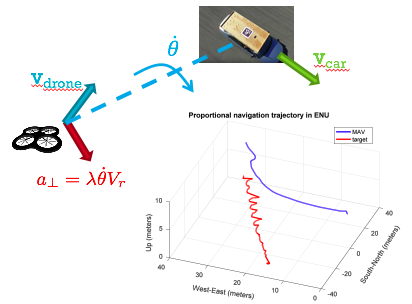
\includegraphics[width=\textwidth]{figures/PNpic.png}\\
            %\caption{Truck based long range MAV deployments}
            %Truck based long range MAV deployments
            %\label{fig:b}
         \end{minipage}


	%Proportional Navigation 
	%\begin{align*}
	%	a_{\perp} = - \lambda |\dot{u}| \frac{u}{|u|} \times \Omega,
%\; \text{with } \Omega = \frac{u \times \dot{u}}{u \cdot u},
	%\end{align*}
	\begin{enumerate}
	\item[$a_{\perp}$] Commanded acceleration normal to the LOS %MAV's velocity
	\item[$\lambda$] Navigation gain
	\item[$u$] Relative position of the car w.r.t the MAV (in 2D)
	\item[$\dot{u}$] Relative velocity of the car w.r.t. the MAV (in 2D)
	\end{enumerate}
\end{frame}

% ----------------------------------------------------------------------

%\begin{frame}{\thesection. \insertsection \ - \insertsubsection}
%	Why True Proportional Navigation?
%	\begin{enumerate}
%		\item Simplest variant of Proportional Navigation that worked
%		\item Car is assumed to move close to constant velocity
%	\end{enumerate}
%\end{frame}

% ----------------------------------------------------------------------

\begin{frame}{\thesection. \insertsection \ - \insertsubsection}
	Approach velocity PD control
	\begin{align}
		a_\parallel = K_{p\parallel} u + K_{d\parallel} \dot{u} 
	\end{align}
	\begin{enumerate}
		\item[$a_\parallel$] Acceleration parallel to the line of sight
		\item[$K_{p\parallel}$, $K_{d\parallel}$] Constant proportional and derivative gains
		\item[$u$] Relative position of the car w.r.t the MAV
		\item[$\dot{u}$] Relative velocity of the car w.r.t. the MAV \textit{projected on the line of sight vector}
	\end{enumerate}
\end{frame}

% ----------------------------------------------------------------------

%\begin{frame}{\thesection. \insertsection \ - \insertsubsection}
%	The complete controller is the combination of both acceleration components
%	\begin{align}
%		a = a_\perp + a_\parallel
%	\end{align}
%	We only navigate horizontally, thus the $z$-axis is disregarded.
%\end{frame}

% ----------------------------------------------------------------------

\begin{frame}{Proportional Navigation Guidance Example}

\begin{center}
\includemedia[
			%width=0.4\linewidth,
	  		%totalheight=0.225\linewidth,
	  		activate=pageopen,
			%final,
			playbutton=plain, %none,
	  		passcontext,  %show VPlayer's right-click menu
	  		addresource=figures/PN.mp4,
	  		flashvars={
	    		%important: same path as in `addresource'
	    		source=figures/PN.mp4
			}
		]{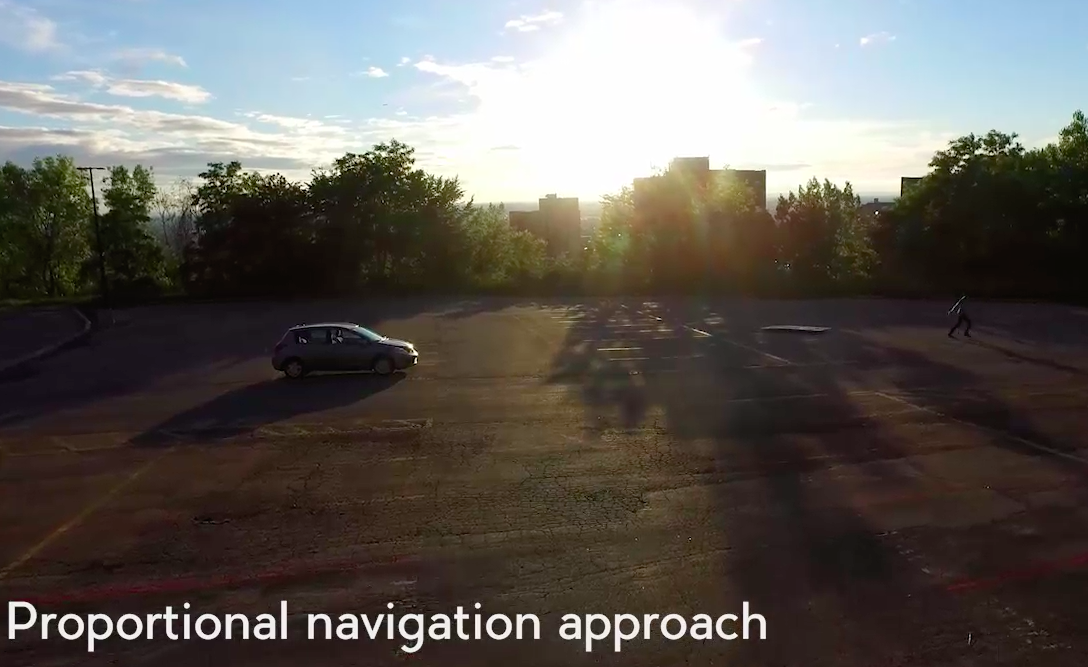
\includegraphics[width=\textwidth]{figures/PNposter.png}}{VPlayer.swf}
\end{center}

\end{frame}



%\subsection{Close Range Controller}

%\begin{frame}{\thesection. \insertsection \ - \insertsubsection}
\begin{frame}{Close Range Controller}
	At close range, we switch the controller
	\begin{enumerate}
		\item Horizontal control : PD controller to match the velocity of the GV
	\begin{align*}
		a = K_p u + K_d \dot{u}
	\end{align*}
%	\begin{enumerate}
%		\item[$a$] MAV acceleration
%		\item[$K_p$, $K_d$] Proportional and derivative gain
%		\item[$u$] Relative position of the car w.r.t. the MAV 
%	\end{enumerate}
	$a$ = MAV acceleration \\
	$K_p$, $K_d$ proportional and derivative gain \\
	$u$ relative position of the GV w.r.t. the MAV
		\item Vertical control : constant descent velocity
	\end{enumerate} 
\end{frame}

% ----------------------------------------------------------------------

%\begin{frame}{\thesection. \insertsection \ - \insertsubsection}
\begin{frame}{Final Descent}
	%\begin{figure}
		\begin{center}
		%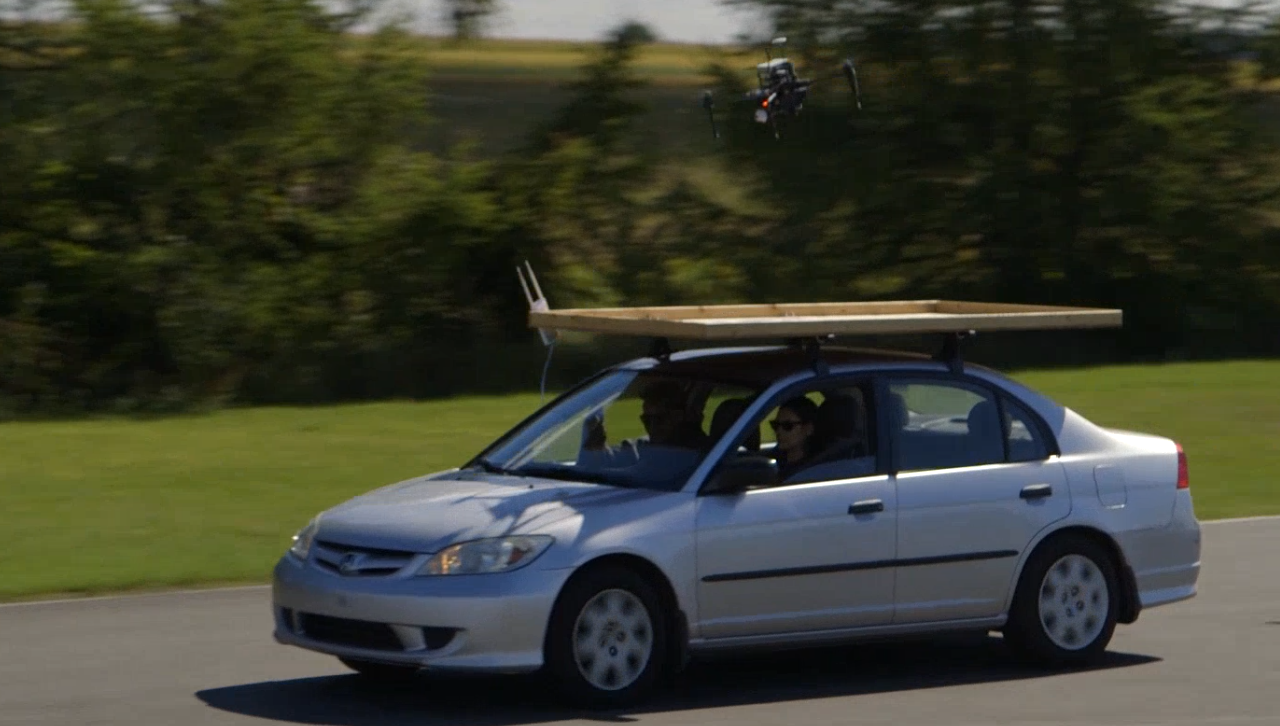
\includegraphics[width=0.7\paperwidth]{figures/landing.png} \\
		%\begin{frame}
		%	\movie{figures/landing.png}{figures/touchdown.mp4}
		%\end{frame}
		%\caption{
		%}
		\includemedia[
			%width=0.4\linewidth,
	  		%totalheight=0.225\linewidth,
	  		%activate=pageopen,
			%final,
			playbutton=plain, %none,
	  		passcontext,  %show VPlayer's right-click menu
	  		addresource=figures/touchdown.mp4,
	  		flashvars={
	    		%important: same path as in `addresource'
	    		source=figures/touchdown.mp4
			}
		]{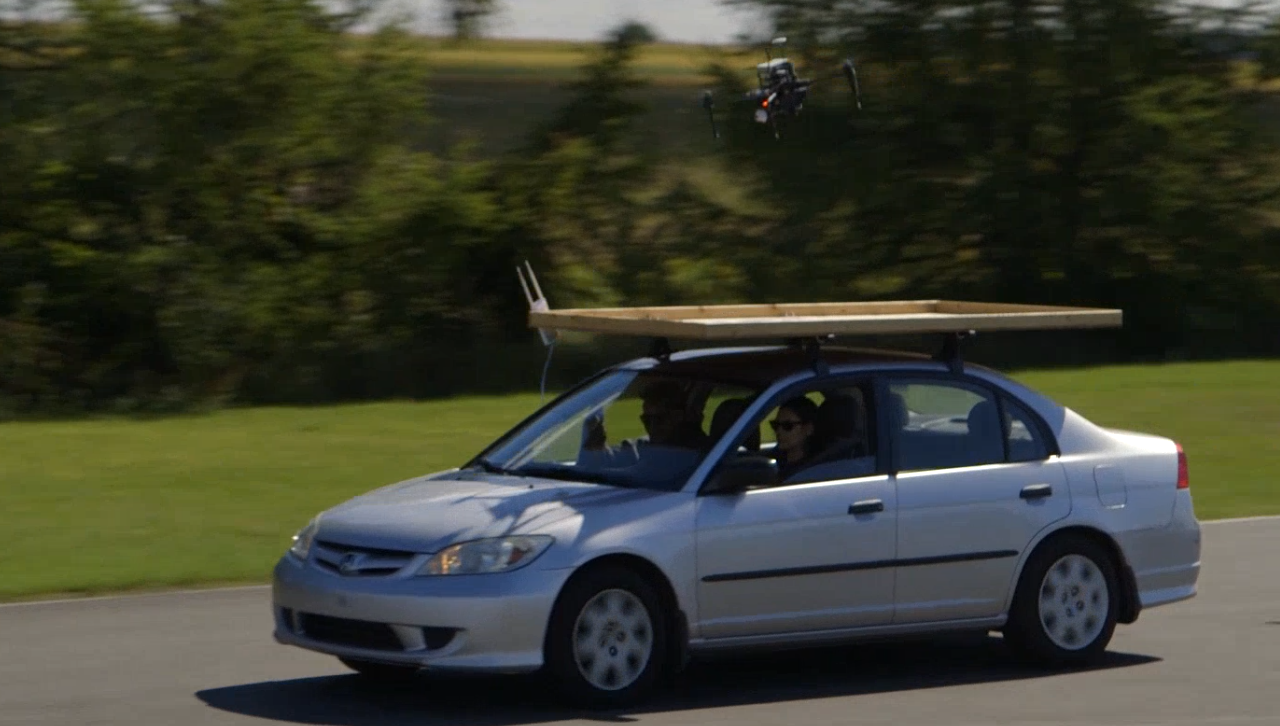
\includegraphics[width=0.7\paperwidth]{figures/landing.png}}{VPlayer.swf}
		%{\fbox{Click!}}{VPlayer.swf}
		\end{center}
\begin{itemize}
	\item Start descent when MAV stable over the landing platform 
	\item Constant vertical velocity %is applied. 
	\item At $0.2$ m: straighten out attitude and cut motors off
	%\end{figure}
\end{itemize}
\end{frame}


% ----------------------------------------------------------------------

%\subsection{Controller Switching}

%\begin{frame}{\thesection. \insertsection \ - \insertsubsection}
\begin{frame}{Controller Switching}
	\begin{itemize}
	\item Switch from long range PN to close range PD at distance $\sim 6-7$ m
	\vspace{0.5cm}
	\item Different sensors used (discard optical flow above GV)
	\vspace{0.5cm}
	\item Switching condition and distance tuned such that
	\begin{enumerate}
		\item Visual detection of the AprilTag is acquired
		\item Outputs of both controllers are similar
	\end{enumerate}
%	\item In practice, 
	\end{itemize}
	
\end{frame}

% ----------------------------------------------------------------------